\documentclass{article}

\usepackage{graphicx}
\usepackage{tikz}
\usepackage{tikzsymbols}
\usetikzlibrary{calc,patterns,shapes.geometric}
\pagestyle{empty}
\usepackage[margin=0pt]{geometry}
\geometry{papersize={14in,12in}}

\def\centerarc[#1](#2)(#3:#4:#5){\draw[#1] ($(#2)+({#5*cos(#3)},{#5*sin(#3)})$) arc (#3:#4:#5);}

\begin{document}
	\begin{figure}
		\centering
		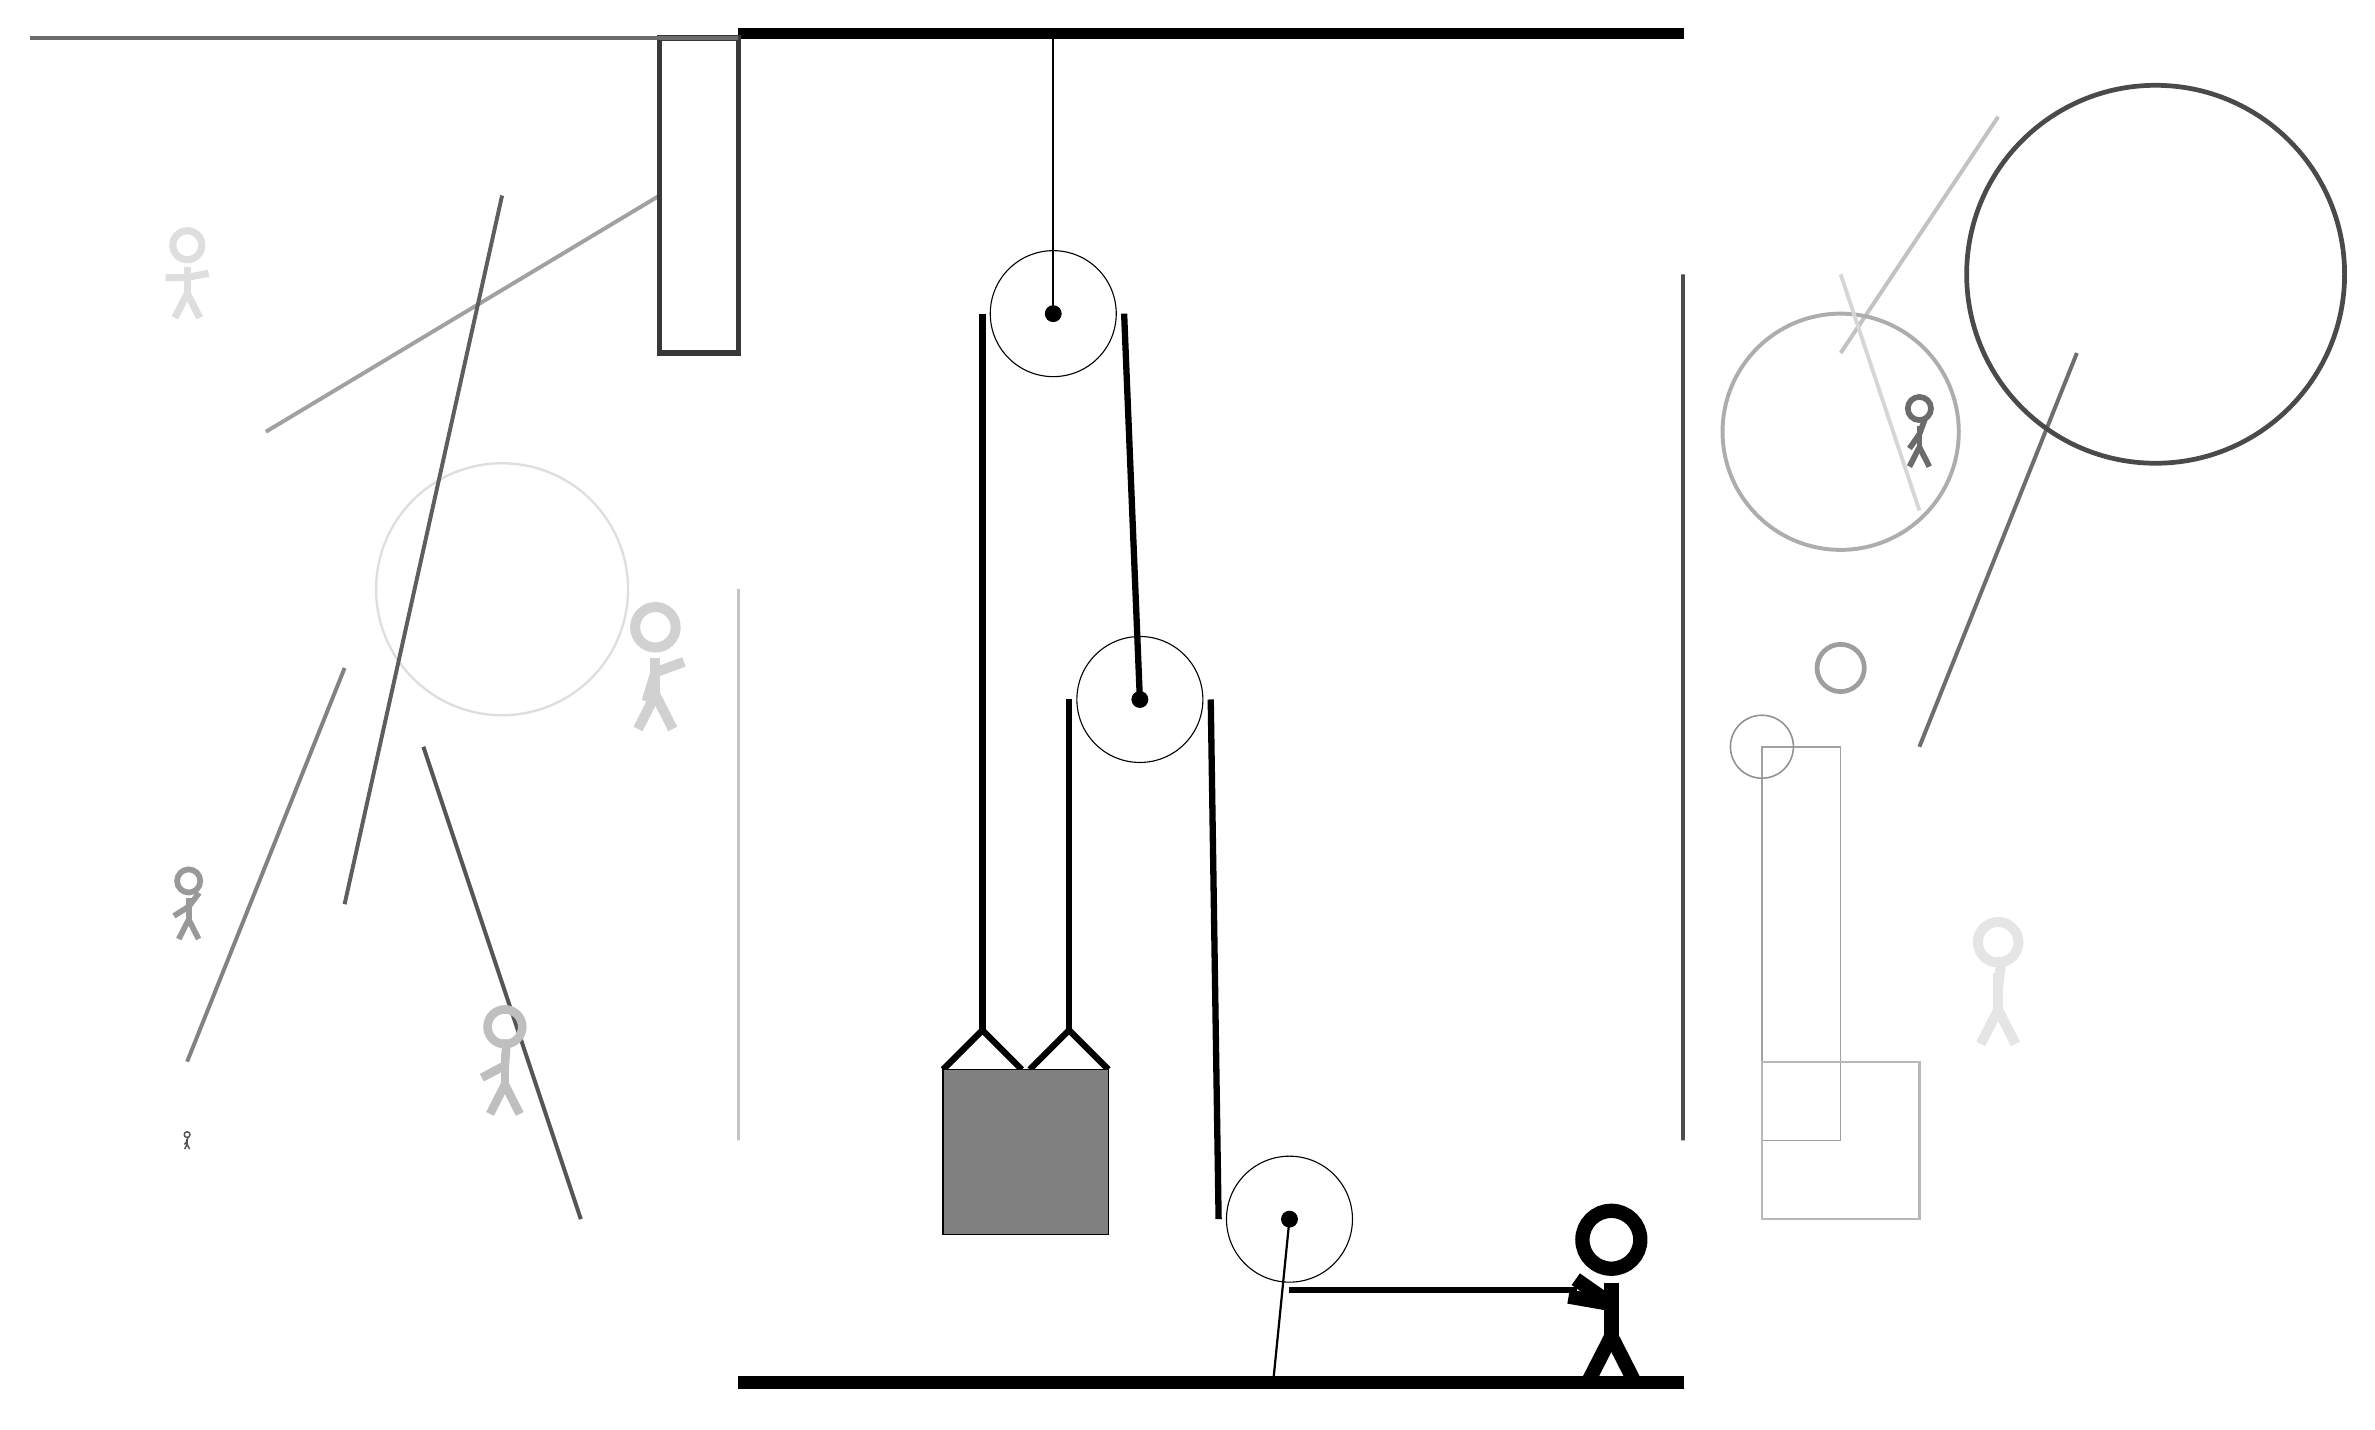
\begin{tikzpicture}
			%%%%% START %%%%%
			
			\draw[fill=black] (-2, 14) rectangle (10, 14.125);
			
			\draw (2, 10.5) circle (0.8);
			\draw[fill=black] (2, 10.5) circle (0.1);
			\draw[thick] (2, 10.5) -- (2, 14);
			
			\draw[line width=0.2mm, color=black!37] (11, 5) rectangle (12, 0);
			
			\draw[line width=0.5mm, color=black!67](-6, 5) -- (-4, -1);
			\draw[line width=0.5mm, color=black!49](-7, 6) -- (-9, 1);
			\draw [line width=0.2mm, color=black!43](11, 5) circle (0.4);
			
			\node[line width=0.2mm, color=black!10] at (14, 2) {\Strichmaxerl[7][90][83]};
			
			\node[line width=0.3mm, color=black!18] at (-3, 6) {\Strichmaxerl[7][73][20]};
			\draw [line width=0.3mm, color=black!13](-5, 7) circle (1.6);
			\node[line width=0.2mm, color=black!25] at (-5, 1) {\Strichmaxerl[6][28][86]};
			\draw[line width=0.5mm, color=black!37](-3, 12) -- (-8, 9);
			\draw[line width=0.5mm, color=black!70] (10, 11) rectangle (10, 0);
			
			\node[line width=0.6mm, color=black!68] at (-9, 0) {\Strichmaxerl[1][52][80]};
			\draw[line width=0.7mm, color=black!78] (-2, 10) rectangle (-3, 14);
			\draw[line width=0.4mm, color=black!23] (-2, 7) rectangle (-2, 0);
			
			\draw[line width=0.5mm, color=black!24](12, 10) -- (14, 13);
			\node[line width=0.5mm, color=black!40] at (-9, 3) {\Strichmaxerl[4][32][53]};
			\draw[line width=0.5mm, color=black!57](15, 10) -- (13, 5);
			
			\draw [line width=0.6mm, color=black!38](12, 6) circle (0.3);
			\node[line width=0.5mm, color=black!58] at (13, 9) {\Strichmaxerl[4][55][70]};
			\draw [line width=0.6mm, color=black!71](16, 11) circle (2.4);
			\draw [line width=0.5mm, color=black!32](12, 9) circle (1.5);
			\node[line width=0.3mm, color=black!13] at (-9, 11) {\Strichmaxerl[5][1][11]};
			
			\draw[line width=0.5mm, color=black!58](-2, 14) -- (-11, 14);
			
			\draw[line width=0.3mm, color=black!28] (11, -1) rectangle (13, 1);
			\draw[line width=0.5mm, color=black!16](13, 8) -- (12, 11);
			\draw[line width=0.5mm, color=black!63](-5, 12) -- (-7, 3);
			
			
			\draw (3.1, 5.6) circle (0.8);
			\draw[fill=black] (3.1, 5.6) circle (0.1);
			
			\draw (5, -1) circle (0.8);
			\draw[fill=black] (5, -1) circle (0.1);
			\draw[thick] (5, -1) -- (4.8, -3);
			
			\draw[line width = 0.8mm]  (0.6, 0.9) -- (1.1, 1.4) -- (1.6, 0.9);
			\draw[line width = 0.8mm]  (1.7, 0.9) -- (2.2, 1.4) -- (2.7, 0.9);
			\draw[fill=black!50] (0.6, 0.9) rectangle (2.7, -1.2);
			
			\draw[line width = 0.8mm] (1.1, 10.5) -- (1.1, 1.4);
			\centerarc[line width = 0.8mm](2, 10.5)(0:180:0.9);
			\draw[line width = 0.8mm] (2.9, 10.5) -- (3.1, 5.6);
			\draw[line width = 0.8mm] (2.2, 5.6) -- (2.2, 1.4);
			\centerarc[line width = 0.8mm](3.1, 5.6)(0:180:0.9);
			\draw[line width = 0.8mm] (4.0, 5.6) -- (4.1, -1);
			\centerarc[line width = 0.8mm](5, -1)(180:270:0.9);
			\draw[line width = 0.8mm] (5, -1.9) -- (8.65, -1.9);
			
			\node at (9, -2) {\Strichmaxerl[10][-35][170]};
			
			\draw[fill=black] (-2, -3) rectangle (10, -3.15);
			
			%%%%% END %%%%%
		\end{tikzpicture}
	\end{figure}	
\end{document}